\documentclass[a4paper,UTF8]{article}
\usepackage{ctex}
\usepackage[margin=1.25in]{geometry}
\usepackage{color}
\usepackage{graphicx}
\usepackage{amssymb}
\usepackage{amsmath}
\usepackage{amsthm}
\usepackage{enumerate}
\usepackage{bm}
\usepackage{hyperref}
\usepackage{epsfig}
\usepackage{color}
\usepackage{tcolorbox}
\usepackage{mdframed}
\usepackage{lipsum}
\usepackage{bbm}
\newmdtheoremenv{thm-box}{myThm}
\newmdtheoremenv{prop-box}{Proposition}
\newmdtheoremenv{def-box}{定义}



\setlength{\evensidemargin}{.25in}
\setlength{\textwidth}{6in}
\setlength{\topmargin}{-0.5in}
\setlength{\topmargin}{-0.5in}
% \setlength{\textheight}{9.5in}
%%%%%%%%%%%%%%%%%%此处用于设置页眉页脚%%%%%%%%%%%%%%%%%%
\usepackage{fancyhdr}                                
\usepackage{lastpage}                                           
\usepackage{layout}                                             
\footskip = 10pt 
\pagestyle{fancy}                    % 设置页眉                 
\lhead{2018年春季}                    
\chead{机器学习导论}                                                
% \rhead{第\thepage/\pageref{LastPage}页} 
\rhead{作业一}                                                                                               
\cfoot{\thepage}                                                
\renewcommand{\headrulewidth}{1pt}  			%页眉线宽,设为0可以去页眉线
\setlength{\skip\footins}{0.5cm}    			%脚注与正文的距离           
\renewcommand{\footrulewidth}{0pt}  			%页脚线宽,设为0可以去页脚线

\makeatletter 									%设置双线页眉                                        
\def\headrule{{\if@fancyplain\let\headrulewidth\plainheadrulewidth\fi%
\hrule\@height 1.0pt \@width\headwidth\vskip1pt	%上面线为1pt粗  
\hrule\@height 0.5pt\@width\headwidth  			%下面0.5pt粗            
\vskip-2\headrulewidth\vskip-1pt}      			%两条线的距离1pt        
 \vspace{6mm}}     								%双线与下面正文之间的垂直间距              
\makeatother  

%%%%%%%%%%%%%%%%%%%%%%%%%%%%%%%%%%%%%%%%%%%%%%
\numberwithin{equation}{section}
%\usepackage[thmmarks, amsmath, thref]{ntheorem}
\newtheorem{myThm}{myThm}
\newtheorem*{myDef}{Definition}
\newtheorem*{mySol}{Solution}
\newtheorem*{myProof}{Proof}
\newcommand{\indep}{\rotatebox[origin=c]{90}{$\models$}}
\newcommand*\diff{\mathop{}\!\mathrm{d}}

\usepackage{multirow}

%--

%--
\begin{document}
\title{机器学习导论\\
作业一}
\author{151250189, 翟道京, zhaidj@smail.nju.edu.cn}
\maketitle

\section*{学术诚信}

本课程非常重视学术诚信规范,助教老师和助教同学将不遗余力地维护作业中的学术诚信规范的建立。希望所有选课学生能够对此予以重视。\footnote{参考尹一通老师\href{http://tcs.nju.edu.cn/wiki/}{高级算法课程}中对学术诚信的说明。}

\begin{tcolorbox}
\begin{enumerate}
  \item[(1)] 允许同学之间的相互讨论,但是{\color{red}\textbf{署你名字的工作必须由你完成}},不允许直接照搬任何已有的材料,必须独立完成作业的书写过程;
  \item[(2)] 在完成作业过程中,对他人工作(出版物、互联网资料)中文本的直接照搬(包括原文的直接复制粘贴及语句的简单修改等)都将视为剽窃,剽窃者成绩将被取消。{\color{red}\textbf{对于完成作业中有关键作用的公开资料,应予以明显引用}};
  \item[(3)] 如果发现作业之间高度相似将被判定为互相抄袭行为,{\color{red}\textbf{抄袭和被抄袭双方的成绩都将被取消}}。因此请主动防止自己的作业被他人抄袭。
\end{enumerate}
\end{tcolorbox}

\section*{作业提交注意事项}
\begin{tcolorbox}
\begin{enumerate}
  \item[(1)] 请严格参照课程网站作业提交方法一节提交作业;
  \item[(2)] 未按照要求提交作业,或提交作业格式不正确,将会被扣除部分作业分数;
  \item[(3)] 除非有特殊情况(如因病缓交),否则截止时间后不接收作业,本次作业记零分。
\end{enumerate}
\end{tcolorbox}

\newpage
\section{[25pts] Basic Probability and Statistics}
随机变量$X$的概率密度函数如下,
\begin{equation}
	f_X(x) = 
	\begin{cases}
		\frac{1}{4} & 0<x<1;\\
		\frac{3}{8} & 3<x<5;\\
		0			& \mbox{otherwise.}
	\end{cases}
\end{equation}
\begin{enumerate}[ {(}1{)}]
\item \textbf{[5pts]} 请计算随机变量$X$的累积分布函数$F_X(x)$;
\item \textbf{[10pts]} 随机变量$Y$定义为$Y = 1/X$,求随机变量$Y$对应的概率密度函数$f_Y(y)$;
\item \textbf{[10pts]} 试证明,对于非负随机变量$Z$,如下两种计算期望的公式是等价的。
\begin{equation}
	\label{eq-expect-1}
	\mathbb{E}[Z] = \int_{z=0}^{\infty}zf(z) \diff z.
\end{equation}

\begin{equation}
	\label{eq-expect-2}
	\mathbb{E}[Z] = \int_{z=0}^{\infty}\Pr[Z\geq z] \diff z.
\end{equation}

同时,请分别利用上述两种期望公式计算随机变量$X$和$Y$的期望,验证你的结论。
\end{enumerate}
\begin{mySol}
\begin{enumerate}[ {(}1{)}]

%1.1
\item 累计算随机变量X的累积分布函数$F_X(x)$定义为 
\begin{equation}
F_X(x) = P(X \leq x) = \int_{-\infty}^{x} f_X(t) dt 
\end{equation}
得
\begin{equation}
	F_X(x) = 
	\begin{cases}
		0 & x \leq 0;\\
		\frac{1}{4}x & 0<x\leq1;\\
		\frac{1}{4} &1<x\leq 3;\\
		\frac{1}{4}+\frac{3}{8}(x-3) & 3<x<5; \\
		1 & x>5.
	\end{cases}
\end{equation}

%1.2
\item 根据随机变量Y的定义:$Y = 1/X$,首先讨论y的取值

\begin{equation}
	\begin{cases}
		F_Y(y) = P(Y<y) = P(\frac{1}{X} < y) = P(\frac{1}{y} < X<0) = F_X(0) - F_X(\frac{1}{y}) = 0 & y<0;\\
		F_Y(y) = 0 & y=0;\\
		F_Y(y) = P(Y<y) = P(\frac{1}{X} < y) = P(X> \frac{1}{y} )  = 1-	F_X(\frac{1}{y})		& y>0
	\end{cases}
\end{equation}
对$y>0$,可获得累计分布函数$F_Y(y)$为
\begin{equation}
	F_Y(y) = 
	\begin{cases}
		1- \frac{1}{4y} & y>1;\\
		\frac{3}{4} & \frac{1}{3}<y <1;\\
		\frac{15}{8}-\frac{3}{8y} & \frac{1}{5}<y<\frac{1}{3};\\
		0			& 0 <y<\frac{1}{5}.
	\end{cases}
\end{equation}
根据$F_Y'(y) = f_Y(y)$,概率密度函数$f_Y(y)$为
\begin{equation}
	f_Y(y) = 
	\begin{cases}
		\frac{1}{4y^2} & y>1;\\
		\frac{3}{8y^2} & \frac{1}{5}<y<\frac{1}{3};\\
		0			& \mbox{otherwise.}
	\end{cases}
\end{equation}

%1.3
\item 在几何分布章节内,我们学过离散化形式的类似公式:

对非负整数型随机变量$Z$,满足
\[ \mathbb{E}[Z] = \sum_{i=1}^{\infty} P (Z \geq i) \].
这里将类似公式推导到连续性随机变量,讲随机变量$Z$写为积分形式,对$\forall \omega \in \Omega$ 
\[ Z(\omega) = \int_{0}^{Z(\omega)} \diff z = \int_{0}^{\infty} \mathbbm{1}_{(0\leq z \leq Z(\omega))}(z) \diff z \] 
期望表达式为
\begin{align*}
\mathbb{E}[Z]  = \int_{\Omega} Z \diff P = \int_{\Omega} \int_{0}^{\infty} \mathbbm{1}_{(0\leq z \leq Z)}(z) \diff z \diff P
\end{align*}
变换积分顺序,得到
\begin{align*}
\mathbb{E}[Z] &  =\int_{0}^{\infty} \int_{\Omega}  \mathbbm{1}_{(0\leq z \leq Z)}(z)  \diff P \diff z \\
& = \int_{0}^{\infty} Pr[Z \geq z] \diff z
\end{align*}
同时根据$\diff P = f(z)$,得到
\[ \mathbb{E}[Z] = \int_{\Omega} Z \diff P = \int_{z=0}^{\infty}zf(z) \diff z \]
因此得证两种表达形式是等价的。


下面我们进行验证,用第一种方法计算
\[ \mathbb{E}[X] = \int_{x=0}^{\infty} f_X(x) \diff x=   \int_{0}^{1} \frac{1}{4}x \diff x + \int_{3}^{5} \frac{3}{8}x \diff x = \frac{25}{8} \]
\[\mathbb{E}[Y] = \int_{y=0}^{\infty} f_Y(y) \diff y=   \int_{\frac{1}{5}}^{\frac{1}{3}} \frac{3}{8y} \diff y+ \int_{1}^{\infty} \frac{1}{4y} \diff y = \infty  \]
用第二种方法来计算
\[ \mathbb{E}[X] = \int_{x=0}^{\infty}\Pr[X\geq x] \diff x =  \int_{0}^{1} (1-\frac{1}{4}x) \diff x + \int_{1}^{3} \frac{3}{4} \diff x + \int_{3}^{5} (\frac{1}{8} - \frac{3}{8}x) \diff x = \frac{25}{8} \]
\[ \mathbb{E}[Y] = \int_{y=0}^{\infty}\Pr[Y\geq y] \diff y =  \int_{0}^{\frac{1}{5}} 1 \diff y + \int_{\frac{1}{5}}^{\frac{1}{3}} (\frac{3}{8y}-\frac{7}{8}) \diff y + \int_{\frac{1}{3}}^{1}\frac{1}{4} \diff y + \int_{1}^{\infty} \frac{1}{4y} \diff y= \infty \] 
从而得以验证。




\end{enumerate}
\end{mySol}

\newpage

\section{[20pts] Strong Convexity}
通过课本附录章节的学习,我们了解到凸性(convexity)对于机器学习的优化问题来说是非常良好的性质。下面,我们将引入比凸性还要好的性质——强凸性(strong convexity)。
\begin{def-box}[强凸性]
记函数$f: \mathcal{K} \rightarrow \mathbb{R}$,如果对于任意$\mathbf{x}, \mathbf{y} \in \mathcal{K}$及任意$\alpha\in[0,1]$,有以下命题成立
\begin{equation}
  \label{eq-sc-1}
  f((1-\alpha)\mathbf{x} + \alpha\mathbf{y})\leq (1-\alpha)f(\mathbf{x}) + \alpha f(\mathbf{y}) - \frac{\lambda}{2}\alpha(1-\alpha)\lVert \mathbf{x} - \mathbf{y}\rVert^2.
\end{equation}
则我们称函数$f$为关于范数$\lVert \cdot \rVert$的$\lambda$-强凸函数。
\end{def-box}

请证明,在函数$f$可微的情况下,式~\eqref{eq-sc-1}与下式~\eqref{eq-sc-2}等价,
\begin{equation}
  \label{eq-sc-2}
  f(\mathbf{y}) \geq f(\mathbf{x}) + \nabla f(\mathbf{x})^\mathrm{T}(\mathbf{y}-\mathbf{x}) + \frac{\lambda}{2}\lVert \mathbf{y} - \mathbf{x}\rVert^2.
\end{equation}

\begin{myProof}

如果式~\eqref{eq-sc-1}与式~\eqref{eq-sc-2}中范数为$\lVert \cdot \rVert_2$,我们可以借助辅助函数来证明两式等价\footnote{参考\href{http://xingyuzhou.org/blog/notes/strong-convexity}{Xingyu Zhou博客中对于Strong convexity性质的研究}}。

记$g(\mathbf{x}) = f(\mathbf{x}) - \frac{\lambda}{2} \rVert \mathbf{x} \rVert ^2_2$,我们下面证明三个命题等价\\
(1) $g(\mathbf{x})$ 为凸函数(convex function) \\
(2) $ f((1-\alpha)\mathbf{x} + \alpha\mathbf{y})\leq (1-\alpha)f(\mathbf{x}) + \alpha f(\mathbf{y}) - \frac{\lambda}{2}\alpha(1-\alpha)\lVert \mathbf{x} - \mathbf{y}\rVert^2_2.$ \\
(3)  $f(\mathbf{y}) \geq f(\mathbf{x}) + \nabla f(\mathbf{x})^\mathrm{T}(\mathbf{y}-\mathbf{x}) + \frac{\lambda}{2}\lVert \mathbf{y} - \mathbf{x}\rVert^2_2.$


首先证明$(1) \Leftrightarrow (2)$:
若$g(\mathbf{x})$为凸函数,根据凸函数的定义,$g(\mathbf{x})$满足
\[ g((1-\alpha)\mathbf{x}+\alpha\mathbf{y}) \leq (1-\alpha)g(\mathbf{x}) + \alpha g(\mathbf{y}) \]
即
\[ f((1-\alpha)\mathbf{x}+\alpha\mathbf{y}) - \frac{\lambda}{2}  \rVert (1-\alpha)\mathbf{x}+\alpha\mathbf{y} \rVert ^2_2 \leq (1-\alpha)(f(\mathbf{x}) - \frac{\lambda}{2} \rVert \mathbf{x} \rVert ^2_2) + \alpha(f(\mathbf{y}) - \frac{\lambda}{2} \lVert \mathbf{y} \rVert ^2_2) \]
化简得到
\[ f((1-\alpha)\mathbf{x}+\alpha\mathbf{y}) \leq (1-\alpha)f(\mathbf{x}) + \alpha f(\mathbf{y}) +\frac{\lambda}{2}  \lVert (1-\alpha)\mathbf{x}+\alpha\mathbf{y} \rVert ^2_2- \frac{(1-\alpha) \lambda}{2} \rVert \mathbf{x} \rVert ^2_2 -\frac{\alpha \lambda}{2} \lVert \mathbf{y} \rVert ^2_2 \]
其中对$\lVert \cdot \rVert_2$有
\[ \frac{\lambda}{2}  \lVert (1-\alpha)\mathbf{x}+\alpha\mathbf{y} \rVert ^2_2 - \frac{(1-\alpha) \lambda}{2} \lVert \mathbf{x} \rVert ^2_2 -\frac{\alpha \lambda}{2} \lVert \mathbf{y} \rVert ^2_2 = \frac{\lambda}{2}\alpha(1-\alpha)\lVert \mathbf{x} - \mathbf{y}\rVert^2_2 \]
因此得到
\[ f((1-\alpha)\mathbf{x} + \alpha\mathbf{y})\leq (1-\alpha)f(\mathbf{x}) + \alpha f(\mathbf{y}) - \frac{\lambda}{2}\alpha(1-\alpha)\lVert \mathbf{x} - \mathbf{y}\rVert^2_2. \]
即证得$(1) \Leftrightarrow (2)$。

\newpage
下面我们证明$(1) \Leftrightarrow (3)$,这里我们使用1st-order condition \footnote{参考\href{https://see.stanford.edu/materials/lsocoee364a/03convexfunctions.pdf}{Boyd \& Vandenberghe. Stanford Convex Optimization.}} 

\begin{prop-box}[1st-order condition]
 Differentiable f with convex domain is convex if and only if 
\[ f( \mathbf{y}) \geq f( \mathbf{x}) + \nabla f( \mathbf{x})^T( \mathbf{y}- \mathbf{x}) ~~for ~all ~\mathbf{x}, \mathbf{y} \in \mathbf{dom} f \]
 \end{prop-box}
 
显然对凸函数 $g( \mathbf{x}) $,根据1st-order condition,得到
\[ f(\mathbf{y}) - \frac{\lambda}{2} \lVert \mathbf{y} \rVert ^2_2 \geq  f(\mathbf{x}) - \frac{\lambda}{2} \lVert \mathbf{x} \rVert ^2_2 + \nabla (f(\mathbf{x}) - \frac{\lambda}{2} \lVert \mathbf{x} \rVert ^2_2)^T (  \mathbf{y} - \mathbf{x}) \]
化简得到
\[ f(\mathbf{y}) \geq f(\mathbf{x}) + \frac{\lambda}{2} \lVert \mathbf{y} \rVert ^2_2 - \frac{\lambda}{2} \lVert \mathbf{x} \rVert ^2_2 + \nabla (f(\mathbf{x}) - \frac{\lambda}{2} \lVert \mathbf{x} \rVert ^2_2)^T (  \mathbf{y} - \mathbf{x}) \]
整理得

\begin{align*}
f(\mathbf{y}) &\geq f(\mathbf{x}) + \nabla f(\mathbf{x})^\mathrm{T}(\mathbf{y}-\mathbf{x}) + \frac{\lambda}{2}(\lVert \mathbf{y} \rVert ^2_2 - \lVert \mathbf{x} \rVert ^2_2  - \nabla (\lVert \mathbf{x} \rVert ^2_2)^\mathrm{T}(\mathbf{y}-\mathbf{x})  )  \\
& = f(\mathbf{x}) + \nabla f(\mathbf{x})^\mathrm{T}(\mathbf{y}-\mathbf{x}) + \frac{\lambda}{2}\lVert \mathbf{y} - \mathbf{x}\rVert^2_2. 
\end{align*} 
其中上式对$f(\mathbf{x}) = \rVert \mathbf{x} \rVert ^2_2 =\mathbf{x}^T \mathbf{x} $ 使用了泰勒展开
\[ f(\mathbf{y}) = f(\mathbf{x}) + \nabla f(\mathbf{x})^\mathrm{T} (\mathbf{y}-\mathbf{x}) + \frac{1}{2}(\mathbf{y}-\mathbf{x})^\mathrm{T} \nabla^2f(\mathbf{z})(\mathbf{y}-\mathbf{x}) \] 

因此证得$(1) \Leftrightarrow (3)$。综上所述,对于$\lVert  \cdot \rVert_2$,式~\eqref{eq-sc-1}与式~\eqref{eq-sc-2}等价。



但是,在上述证明过程中,我们对二范数的运算并不能推广到任意范数,下面我们直接证明~\eqref{eq-sc-1}与式~\eqref{eq-sc-2}等价性。


首先证明$\eqref{eq-sc-1} \to \eqref{eq-sc-2} $,将$\eqref{eq-sc-1} $改写为
\[ \frac{f(\mathbf{x} + \alpha (\mathbf{y} - \mathbf{x})) - f(\mathbf{x})}{\alpha} + \frac{\lambda}{2}(1-\alpha)\lVert \mathbf{x} - \mathbf{y}\rVert^2 \leq f(\mathbf{y}) - f(\mathbf{x}) \]
其中对不等式左边求极限,令$\alpha \to 0^+$
\[ \lim_{\alpha \to 0^+} \left\{\frac{f(\mathbf{x} + \alpha (\mathbf{y} - \mathbf{x})) - f(\mathbf{x})}{\alpha}  +\frac{\lambda}{2}(1-\alpha)\lVert \mathbf{x} - \mathbf{y}\rVert^2 \right\} =   \nabla f(\mathbf{x} )^T (\mathbf{y} - \mathbf{x}) + \frac{\lambda}{2} \lVert \mathbf{x}  - \mathbf{y}\rVert^2\]
从而得到 \eqref{eq-sc-2}
\[ f(\mathbf{y}) \geq f(\mathbf{x}) + \nabla f(\mathbf{x})^\mathrm{T}(\mathbf{y}-\mathbf{x}) + \frac{\lambda}{2}\lVert \mathbf{y} - \mathbf{x}\rVert^2. \]

对于$(2.2) \to (2.1)$,Xingyu Zhou \footnote{\href{https://arxiv.org/pdf/1803.06573.pdf}{Xingyu Zhou, On the Fenchel Duality between Strong Convexity and Lipschitz Continuous Gradient, arxiv}}在对convexity等价条件的证明中使用了一个很巧妙的方式 ,这里我们借鉴这种方式。\\
记
\[ \mathbf{x_\alpha} = (1-\alpha) \mathbf{x} + \alpha \mathbf{y} \]
根据$(2.2)$
\begin{equation}
f(\mathbf{x}) \geq f(\mathbf{x_\alpha}) + \nabla f(\mathbf{x_\alpha})^\mathrm{T}(\mathbf{x}-\mathbf{x_\alpha}) + \frac{\lambda}{2}\lVert \mathbf{x} - \mathbf{x_\alpha}\rVert^2 
\end{equation}

\begin{equation} 
f(\mathbf{y}) \geq f(\mathbf{x_\alpha}) + \nabla f(\mathbf{x_\alpha})^\mathrm{T}(\mathbf{y}-\mathbf{x_\alpha}) + \frac{\lambda}{2}\lVert \mathbf{y} - \mathbf{x_\alpha}\rVert^2 
\end{equation}
考虑$(1-\alpha) (2.3) + \alpha (2.4) $,恰可以得到
\[ f((1-\alpha)\mathbf{x} + \alpha\mathbf{y})\leq (1-\alpha)f(\mathbf{x}) + \alpha f(\mathbf{y}) - \frac{\lambda}{2}\alpha(1-\alpha)\lVert \mathbf{x} - \mathbf{y}\rVert^2 \] 

我们得以证明$(2.1) \Leftrightarrow (2.2)$。
\qed
\end{myProof}


\newpage
\section{[20pts] Doubly Stochastic Matrix}
随机矩阵(stochastic matrix)和双随机矩阵(doubly stochastic matrix)在机器学习中经常出现,尤其是在有限马尔科夫过程理论中,也经常出现在于运筹学、经济学、交通运输等不同领域的建模中。下面给出定义,
\begin{def-box}[随机矩阵]
设矩阵$\mathbf{X}=[x_{ij}]\in \mathbb{R}^{d\times d}$是非负矩阵,如果$\mathbf{X}$满足
\begin{equation}
	\label{eq-sto-matrix}
	\sum_{j=1}^d x_{ij} = 1,\quad i=1,2,\cdots,d.
\end{equation}
则称矩阵$\mathbf{X}$为随机矩阵(stochastic matrix)。如果$\mathbf{X}$还满足
\begin{equation}
	\label{eq-double-sto-matrix}
	\sum_{i=1}^d x_{ij} = 1,\quad j=1,2,\cdots,d.
\end{equation}
则称矩阵$\mathbf{X}$为双随机矩阵(double stochastic matrix)。
\end{def-box}
对于双随机矩阵$\mathbf{X} \in \mathbb{R}^{d\times d}$,试证明
\begin{enumerate}[ {(}1{)}]
\item \textbf{[10pts]} 矩阵$\mathbf{X}$的\href{https://en.wikipedia.org/wiki/Entropy_(information_theory)}{信息熵 (entropy)}满足$H(\mathbf{X}) \leq d\log d$.
\item \textbf{[10pts]} 矩阵$\mathbf{X}$的\href{https://en.wikipedia.org/wiki/Spectral_radius}{谱半径 (spectral radius
)}$\rho(\mathbf{X})$等于1,且是$\mathbf{X}$的特征值;(提示:你可能会需要\href{https://en.wikipedia.org/wiki/Perron%E2%80%93Frobenius_theorem}{Perron–Frobenius定理},可以基于此进行证明。)
\end{enumerate}
\begin{myProof}
(1) 对于矩阵的信息熵为
\begin{equation}
	H(\mathbf{X}) = - \sum_{i=1}^d \sum_{j=1}^d x_{ij} log x_{ij}, \quad i,j = 1,2, \cdots, d.
\end{equation}
其中满足
\[ 	\sum_{i=1}^d x_{ij} = 1,\quad i=1,2,\cdots,d. \]
\[	\sum_{j=1}^d x_{ij} = 1,\quad i=1,2,\cdots,d. \]
对于函数$f(x) = -xlogx$,求二阶导数为
\[ f''(x) = -\frac{1}{xln10} \]
$f''(x)<0$,$f(x)$为凹函数(concave function),同时得到性质
\begin{equation} 
f(\frac{x_1+x_2+\cdots + x_n}{n}) \geq \frac{f(x_1) + f(x_2) +\cdots + f(x_n)}{n} 
\end{equation}
回到我们的问题中,代入公式$(3.4)$,即
\[ f(\frac{1}{d})  \geq \frac{H(\mathbf{X})}{d^2} \]
因而证得$H(\mathbf{X}) \leq d\log d$.

(2) 首先我们进行观察,对于矩阵$\mathbf{X}$,可得到一个特征向量$e = (1,1,\cdots,1)^T$和特征值$\lambda = 1$,满足
\[ \mathbf{X} e = \lambda e \]
因此矩阵的谱半径$\rho(\mathbf{X}) \geq 1$,下面证明$\rho(\mathbf{X}) \leq 1$:\\
根据谱半径的性质:矩阵$\mathbf{A}$的谱半径$\rho(\mathbf{A})$ 不大于任何一种诱导范数\footnote{参考\href{https://en.wikipedia.org/wiki/Spectral_radius}{Wikipedia: Spectral radius}.} ,即
\[ \rho(\mathbf{A}) \leq \lVert \mathbf{A}^k \rVert ^{\frac{1}{k}}  \]
不妨取$k=1$,可得
\begin{equation}
\rho(\mathbf{X}) \leq \lVert \mathbf{X} \rVert_1 = \max_{1 \leq j \leq d} \sum_{i=1}^d |x_{ij} |  = 1
\end{equation}
因为$\rho(\mathbf{X})  \leq 1$ 且 $ \rho(\mathbf{X}) \geq 1 $,所以$\rho(\mathbf{X})=1$

\qed
\end{myProof}
\newpage
\section{[15pts] Hypothesis Testing} 
在数据集$D_1,D_2,D_3,D_4,D_5$运行了$A,B,C,D,E$五种算法,算法比较序值表如表\ref{table:ranking}所示:
\begin{table}[h]
\centering
\caption{算法比较序值表} \vspace{2mm}
\label{table:ranking}
\begin{tabular}{c|c c c c c}\hline
数据集 		& 算法$A$  	&算法$B$  	& 算法$C$ 	& 算法$D$  	&算法$E$ 	\\ \hline
$D_1$ 		& 4 		&  3  		& 5  		&  2 		& 1			\\
$D_2$ 		& 3 		&  5  		& 2  		&  1 		& 4			\\
$D_3$ 		& 4 		&  5  		& 3  		&  1 		& 2			\\ 
$D_4$ 		& 5 		&  2  		& 4  		&  1 		& 3			\\ 
$D_5$ 		& 3 		&  5  		& 2  		&  1 		& 4			\\ \hline
\end{tabular}
\end{table}

使用Friedman检验$(\alpha=0.05)$判断这些算法是否性能都相同。若不相同,进行Nemenyi后续检验$(\alpha=0.05)$,并说明性能最好的算法与哪些算法有显著差别。
\begin{mySol}
首先使用Friedman检验($\alpha = 0.05$)判断这些算法性能是否相同。\\
$A,B,C,D,E$五种算法的平均序值如下表所示

\begin{table}[h]
\centering
\caption{算法比较平均序值表} \vspace{2mm}
\label{table:ranking}
\begin{tabular}{c|c c c c c}\hline
算法 		& 算法$A$  	&算法$B$  	& 算法$C$ 	& 算法$D$  	&算法$E$ 	\\ \hline
平均序值 		& 3.8 		&  4  		& 3.2  		&  1.2 		& 2.8	 \\ \hline
\end{tabular}
\end{table}
根据
\begin{align*}
 \tau_{\chi^2} 	& = \frac{k-1}{k} \cdot \frac{12N}{k^2-1} \sum_{i=1}^{k}(r_i - \frac{k+1}{2})^2 \\
			& = \frac{12N}{k(k+1)} \left ( \sum_{i=1}^{k}r_i^2 - \frac{k(k+1)^2}{4} \right ).
\end{align*}
求得$\tau_{\chi^2}=9.92$,同时根据
\begin{align*}
 \tau_F = \frac{(N-1)\tau_{\chi^2}}{N(k-1)-\tau_{\chi^2}}.
 \end{align*}
 得$ \tau_F = 3.936$,由书上表2.6可知,它大于$\alpha = 0.05$时的$F$检验临界值3.007,因此拒绝“所有算法性能相同这个假设”。\\
然后使用Nemenyi后续检测,在表2.7中找到$k=5$时$q_{0.05}=2.728$,根据下式:
\[ CD = q_\alpha \sqrt{\frac{k(k+1)}{6N}}.
\]
 得到临界值域$CD = 2.728$。相对于性能最好的算法$D$,算法$B$和$D$的差距超过了临界值域,因此两者有显著差距。
\end{mySol}

\newpage
\section{[20pts] ROC and AUC}
现在有五个测试样例,其对应的真实标记和学习器的输出值如表\ref{table:roc}所示:
\begin{table}[!h]
	\centering
	\caption{测试样例表} \vspace{2mm}\label{table:roc}
	\begin{tabular}{c|c c c c c}\hline
		样本 & $x_1$ & $x_2$ & $x_3$  & $x_4$  & $x_5$ \\
		\hline
		标记 & +  & + &  - &  +  & -\\
		\hline
		输出值 & 0.9  & 0.3 &  0.1 &  0.7  & 0.4\\
		\hline
	\end{tabular}
\end{table}
\begin{enumerate}[ {(}1{)}]
\item \textbf{[10pts]} 请画出其对应的ROC图像,并计算对应的$\mbox{AUC}$和$\ell_{rank}$的值(提示:可使用\href{https://en.wikibooks.org/wiki/LaTeX/PGF/TikZ}{TikZ包}作为\LaTeX 中的画图工具);
\item \textbf{[10pts]} 根据书上第35页中的公式(2.20)和公式(2.21),试证明\[\mbox{AUC}+\ell_{rank}=1.\]
\end{enumerate}
\begin{mySol}
(1) 相应的ROC图像如下图所示,
\begin{figure}[!htb]
\centering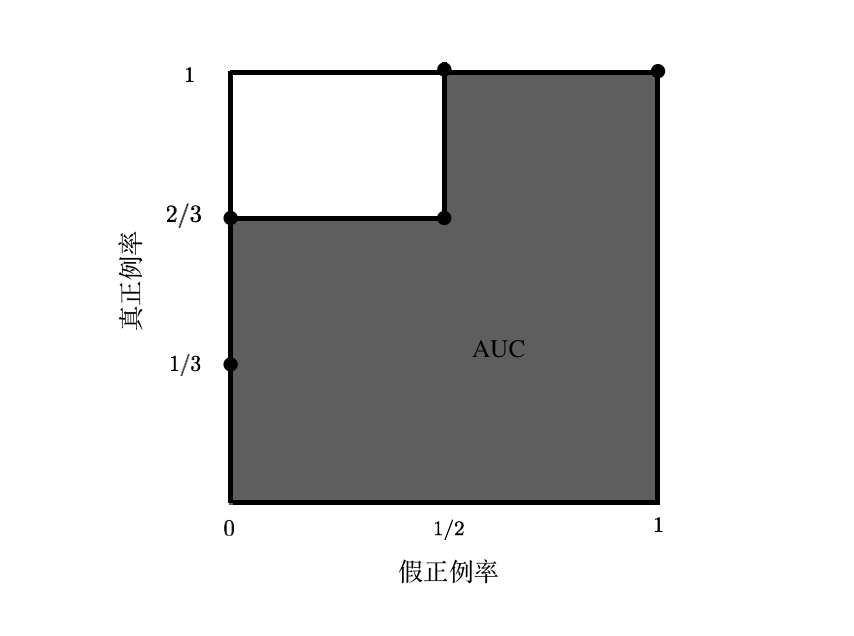
\includegraphics[width = 3.5in] {AUC.jpg}
\caption{ROC曲线与AUC}\label{fig:1}
\end{figure}

显然,根据图像,我们可得$\mbox{AUC} = \frac{5}{6}, \ell_{rank} = \frac{1}{6} $。

(2)我们分两种情况进行讨论:

1) 若无“正例与反例的预测值相同”的情况出现,根据课本中绘制近似ROC曲线的方法,依次判断每个样例,即每次曲线沿横轴延伸$\frac{1}{m^-}$或沿着纵轴延伸$\frac{1}{m^+}$长度。若出现n个正例(或反例)有着相同的预测值,我们分为n步延伸曲线。此时$\ell_{rank}$定义式为
\[ \ell_{rank} = \frac{1}{m^+m^-} \sum_{x^+ \in D^+} \sum_{x^- \in D^-} \left (  \mathbbm{I}(f(x^+)<f(x^-)) \right ). \]
根据课本AUC估算公式(2.20),考虑划分到第$x_{i+1}$个样例的预测值,若$x_{i+1}$为正例,AUC面积未增加;若$x_{i+1}$为反例,此时AUC面积增加$\frac{y_{i+1}}{m^-}$。因此
\[ AUC = \frac{1}{2} \sum_{i=1}^{m-1} (x_{i+1}-x_{i})\cdot (y_i + y_{i+1}) = \frac{1}{m^+m^-} \sum_{x_{i+1} \in D^-}  m^+ y_{i+1} \] 
同时$m^+ y_{i+1} $为前$i+1$个案例中正例的个数,因此
\[ AUC = \frac{1}{m^+m^-} \sum_{x^- \in D^-}  \sum_{x^+ \in D^+} \left (  \mathbbm{I}(f(x^+)>f(x^-)) \right ). \]
此时易得$AUC = 1- \ell_{rank}$。

2) 若存在“正例和反例对应相同的预测值”情况发生。此时如果按照课本上关于ROC曲线绘制的方法一一对样本点进行判定,会出现不同的AUC值(判定正例和负例的顺序不同,AUC值不同),因此我们要进行新的说明:如果出现“正例和反例对应相同的预测值”,在划分该预测值为分类阈值时,一次完成对该预测值下所有样例的延伸,而非一个个点进行处理。

与情况1)相比,我们只需要考虑该特殊情况的发生,若设置某预测值为分类阈值,假设此预测值下有正例k例,负例l例,此步延伸增加的AUC面积为
\[ \Delta AUC = \frac{kl}{2m^+m-} \]
显然地,此时AUC表示为
\[ AUC = \frac{1}{m^+m^-} \sum_{x^- \in D^-}  \sum_{x^+ \in D^+} \left (  \mathbbm{I}(f(x^+)>f(x^-)) + \frac{1}{2}\mathbbm{I}(f(x^+)>f(x^-)) \right ). \] 
这种情况也满足$AUC = 1- \ell_{rank}$。

\end{mySol}

\newpage
\section{[附加题10pts] Expected Prediction Error}
对于最小二乘线性回归问题,我们假设其线性模型为:
\begin{equation}
	y=\textbf{x}^T  \bm{ \beta } + \epsilon , 
\end{equation}
其中$\epsilon$为噪声满足$\epsilon\sim N(0,\sigma^2)$。我们记训练集$\mathcal{D}$中的样本特征为$\textbf{X}\in \mathbb{R}^{p \times n}$,标记为$\textbf{Y}\in \mathbb{R}^{n}$,其中$n$为样本数,$p$为特征维度。
已知线性模型参数的估计为:
\begin{equation}
	\hat{\bm{\beta}}=(\textbf{X}\textbf{X}^T)^{-1}\textbf{X}\textbf{Y}.	
\end{equation}

对于给定的测试样本$\textbf{x}_0$,记$\mathbf{EPE}(\textbf{x}_0)$为其预测误差的期望 (Expected Predication Error),试证明,
\[
	\mathbf{EPE}(\textbf{x}_0) = \sigma^2+\mathbb{E}_{\mathcal{D}}[\textbf{x}_0^T(\textbf{X}\textbf{X}^T)^{-1}\textbf{x}_0\sigma^2].
\]

要求证明中给出详细的步骤与证明细节。(提示:$\mathbf{EPE}(\textbf{x}_0)=\mathbb{E}_{y_0|\textbf{x}_0} \mathbb{E}_{\mathcal{D}}[(y_0-\hat{y}_0)^2]$,可以参考书中第45页关于方差-偏差分解的证明过程。)

\begin{myProof}

\begin{align*}
\mathbf{EPE}(\textbf{x}_0) &= \mathbb{E}_{y_0|\textbf{x}_0} \mathbb{E}_{\mathcal{D}}[(y_0-\hat{y}_0)^2] \\
& = \mathbb{E}_{y_0|\textbf{x}_0} \mathbb{E}_{\mathcal{D}} [((y_0 - \textbf{x}_0^T\bm{\beta} )+( \textbf{x}_0^T\bm{\beta} - \hat{y}_0))^2] \\
& = \mathbb{E}_{y_0|\textbf{x}_0} \mathbb{E}_{\mathcal{D}} [(y_0 - \textbf{x}_0^T\bm{\beta} )^2] +  \mathbb{E}_{y_0|\textbf{x}_0} \mathbb{E}_{\mathcal{D}} [( \textbf{x}_0^T\bm{\beta} - \hat{y}_0)^2] +  \mathbb{E}_{y_0|\textbf{x}_0} \mathbb{E}_{\mathcal{D}} [2(y_0 - \textbf{x}_0^T\bm{\beta} )(\textbf{x}_0^T\bm{\beta} - \hat{y}_0)]
\end{align*}
考虑到$\mathbb{E}_{\mathcal{D}}[\hat{y}_0] = \textbf{x}_0^T\bm{\beta}$,上式第三项为零。因此
\begin{align*}
\mathbf{EPE}(\textbf{x}_0) & = \mathbb{E}_{y_0|\textbf{x}_0} \mathbb{E}_{\mathcal{D}} [(y_0 - \textbf{x}_0^T\bm{\beta} )^2] +  \mathbb{E}_{y_0|\textbf{x}_0} \mathbb{E}_{\mathcal{D}} [( \textbf{x}_0^T\bm{\beta} - \hat{y}_0)^2] \\
& = \mathbb{E}_{y_0|\textbf{x}_0} \mathbb{E}_{\mathcal{D}} [(\epsilon - 0)^2] + \mathbb{E}_{\mathcal{D}} [( \textbf{x}_0^T\bm{\beta} - \hat{y}_0)^2]
\end{align*}
根据噪声$\epsilon$满足$\epsilon\sim N(0,\sigma^2)$,上式第一项为$\sigma^2$,接着
\begin{align*}
\mathbf{EPE}(\textbf{x}_0) & = \sigma^2 + \mathbb{E}_{\mathcal{D}} [( \textbf{x}_0^T\bm{\beta} - \hat{y}_0)^2] \\
& = \sigma^2 + \mathbb{E}_{\mathcal{D}} [(\mathbb{E}_{\mathcal{D}}[\hat{y}_0]-\hat{y}_0)^2] \\
& = \sigma^2 + Var_{\mathcal{D}}[\hat{y}_0]
\end{align*}
根据
\[ \hat{y}_0 = \textbf{x}_0^T \hat{\bm{\beta}},~\hat{\bm{\beta}}=(\textbf{X}\textbf{X}^T)^{-1}\textbf{X}\textbf{Y},~\textbf{Y}=\textbf{X}^T\bm{\beta}+\epsilon \]
带入上式,得到
\begin{align*}
\mathbf{EPE}(\textbf{x}_0) & = \sigma^2 + Var_{\mathcal{D}}[(\textbf{x}_0^T(\textbf{X}\textbf{X}^T)^{-1}\textbf{X}\textbf{Y}] \\
& =  \sigma^2 + \textbf{x}_0^T Var_{\mathcal{D}}[(\textbf{X}\textbf{X}^T)^{-1}\textbf{X}(\textbf{X}^T\bm{\beta}+\epsilon)] \textbf{x}_0\\
& =  \sigma^2 + \textbf{x}_0^T Var_{\mathcal{D}}[\bm{\beta}(\textbf{X}\textbf{X}^T)^{-1}\textbf{X}\textbf{X}^T+\epsilon(\textbf{X}\textbf{X}^T)^{-1}\textbf{X}] \textbf{x}_0 \\
& = \sigma^2 + \textbf{x}_0^T Var_{\mathcal{D}}[\epsilon(\textbf{X}\textbf{X}^T)^{-1}\textbf{X}] \textbf{x}_0
\end{align*}
此时将方差表示为期望形式,可以转化为
\begin{align*}
\mathbf{EPE}(\textbf{x}_0) & = \sigma^2 + \textbf{x}_0^T  \mathbb{E}_{\mathcal{D}} [(\epsilon(\textbf{X}\textbf{X}^T)^{-1}\textbf{X} -  \mathbb{E}_{\mathcal{D}} (\epsilon(\textbf{X}\textbf{X}^T)^{-1}\textbf{X}))^2] \textbf{x}_0 \\
& = \sigma^2 + \textbf{x}_0^T  \mathbb{E}_{\mathcal{D}}[(\epsilon(\textbf{X}\textbf{X}^T)^{-1}\textbf{X})^2]\textbf{x}_0  \\
& = \sigma^2 + \sigma^2 \textbf{x}_0^T  \mathbb{E}_{\mathcal{D}} [((\textbf{X}\textbf{X}^T)^{-1}\textbf{X})^T(\textbf{X}\textbf{X}^T)^{-1}\textbf{X})]\textbf{x}_0 \\
& = \sigma^2+\mathbb{E}_{\mathcal{D}}[\textbf{x}_0^T(\textbf{X}\textbf{X}^T)^{-1}\textbf{x}_0\sigma^2].
\end{align*}

\qed
\end{myProof}




\end{document}